\section{L'échantillonnage}

Après l'acquisition \ref{sec:acquisition}, suivi d'une éventuelle phase de recalage \ref{sec:registration}, la quantité d'informations recueillies peut rapidement croître.

En effet les nuages de points \index{Nuage de points} décrivent souvent des surfaces complexes, et de ce fait, ceux-ci contiennent plusieurs millions, voir des milliards de points~\cite{Levoy}.

En fonction du but recherché, cette masse de données peut handicaper le traitement futur. En effet, beaucoup d'algorithmes de traitement d'image n'ont pas une complexité en $O(n)$ et de ce fait, peuvent être trop lents.

Réduire la complexité de ces nuages de points est une étape importante afin de préparer ces informations à être traités plus ou moins rapidement, en fonction de l'objectif recherché. Le sous-échantillonnage  consiste à déterminer un ensemble de points réduit approchant au mieux le nuage de points original.

Voici une définition possible du sous-échantillonnage \cite{Pauly2003}:

\begin{definition}[Sous-échantillonnage\index{Sous-échantillonnage}]
  Soit $S$ une surface définie par un nuage de points $P$. Soit $n$ le nombre de points dans le nuage sous-échantillonné tel que $n<|P|$.\\
  Le sous-échantillonnage consiste à trouver un nuage de points $P'$ tel que $|P'|=n$ de tel sorte que la distance $\epsilon = d(S,S')$ de la surface correspondante $S'$ à la surface originale $S$ soit minimale.
\end{definition}

Cette définition peut-être inversée, de façon à chercher un sous-ensemble minimal de point tel que la distance entre les deux surfaces $S$ et $S'$ soit minimale.

L'approximation optimale d'une telle surface est un problème \emph{NP-Complet} \cite{Agarwal1994}, et de ce fait, la plupart des recherches dans le domaine sont orientés vers des heuristiques.\\

Afin de faciliter la présentation de différentes méthodes liées au sous-échantillonnage de nuage de points, on distinguera différentes approches ~\cite{Pauly2002}:

\begin{itemize}
  \item Par classification;
  \item Par simplification itérative;
  \item Par simulation de particule.
\end{itemize}

\subsection{Méthode par classification}
\begin{definition}[Sous-échantillonnage par classification]
  Consiste à diviser l'ensemble des points en un ensemble de sous-ensembles notés. Ensuite chacun de ceux-ci est remplacé par un point ou un ensemble de points représentatifs.
\end{definition}

L'objectif est donc d'obtenir un ensemble de classes ${C_i}$ tel que pour tout point $p_j\in P$, il existe une unique classe $C_i$ avec $p_j\in C_i$. $P'$ contiendra donc un point ou un ensemble de points représentatifs pour chaque classe.

Habituellement, on remplacera la classe par sont centre de masse :

$$\overline{p_i}=\frac{1}{|C_i|}\cdot\int_{j\in C_i}p_j$$

Une solution simple permettant d'obtenir des \emph{classes} consiste à diviser la boite englobante du nuage de points en cellules à l'aide d'un maillage régulier. Chacune d'elle contiendra un ensemble de points, qu'il faudra remplacer par un nouveau point représentatif.
Le problème de cette méthode est lié au maillage régulier. En effet, celui-ci ne peut pas s'adapter aux irrégularités de la répartition des points. De plus, si la taille du maillage est trop grande, il est possible que la surface sous-échantillonnée connecte des éléments qui devraient être disjoints.

Afin d'éviter ce genre de problème, il est nécessaire de grouper les points en respectant certains critères liés aux propriétés locales de la surface. Il s'agit d'une étape de \emph{segmentation} \index{segmentation}. \'{A} cette fin, on peut distinguer deux approches:

\begin{itemize}
  \item Incrémentale;
  \item Hiérarchique.
\end{itemize}

\subsubsection{Classification incrémentale}
Ces méthodes se basent sur le principe de \emph{croissance de région} \index{Croissance de région}.

\begin{definition}[Croissance de région]
  Soit un point de démarrage $p_j \in P$, une classe $C_0$ est construite successivement en rajoutant un point respectant une contrainte de similarité.
\end{definition}

La classification consiste à sélectionner un point $p_j$ n'appartenant pas encore à une classe, à effectuer la croissance de région à partir de ce dernier, et s'arrête lorsque tous les points $p_j \in P$ appartiennent à une classe $C_i$.

Généralement, la contrainte sera de minimiser une distance, mais il est possible de cumuler d'autres contraintes. Par exemple, un variation maximum $\sigma_{max}$ de la classe peut être définie. De cette façon, la classification est adaptative à la surface $S$. Une autre contrainte possible consiste à fixer une taille minimum $n_{min}$ et maximum $n_{max}$ aux classes voulues.

$$n_{min} \le |C_i| \le n_{max}$$

De cette façon, les classes peuvent avoir une taille similaire. Afin d'éviter un morcellement trop important, faisant apparaître de trop petites classes, une deuxième phase est nécessaire. Celle-ci rajoute chacun des points $p_j \in C_i$ tel que $|C_i| < n_{min}$ dans la classe la plus proche, tel qu'illustré sur la figure \ref{fig:sampling_incremental_fragmentation}.

\begin{figure}
  \centering
  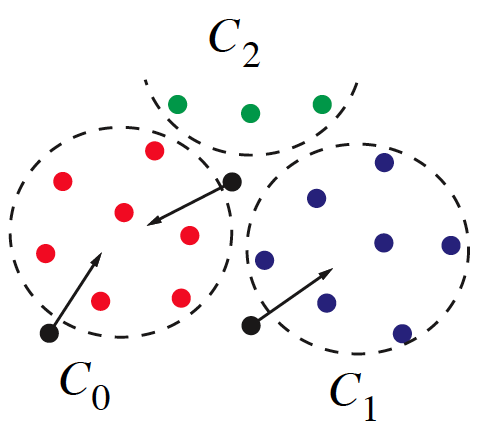
\includegraphics[height=5cm]{incremental_clustering}
  \caption{Morcellement de la classification incrémentale~\cite{Pauly2002} \label{fig:sampling_incremental_fragmentation}}
\end{figure}

\subsubsection{Classification hiérarchique}

La notion hiérarchique fait référence à un procédé de segmentation \emph{division-fusion} exécuté de haut en bas.

\begin{definition}[Division-Fusion (Split and Merge)]
  Méthode de segmentation mêlant un processus de division de classe avec un processus de fusion de classe.
\end{definition}

L'approche de haut en bas signifie que l'ensemble des données est initialement considéré comme une seule classe, et est ensuite divisé si certains critères de similarité ne sont pas respectés. Dans le cas ou deux classes respectent ensemble les critères pré-définis, une nouvelle classe résultera de la fusion de celles-ci.

L'opération de division reste à définir. Pour ce faire, il faut utiliser un \emph{partitionnement binaire de l'espace} (\emph{Binary Space Partitioning} ou \emph{BSP}). L'objectif est de déterminer le plan qui divise l'espace en deux de façon adéquate. Une façon de procéder consiste à définir ce plan par le centre de masse $\overline{p}$ et le vecteur propre $v_i$ issus de la matrice de covariance de $P$, tel que $\lambda_i$ est la plus grande valeur propre. Cette méthode est illustré sur la figure \ref{fig:sampling_hierarchical}

\begin{figure}
  \centering
  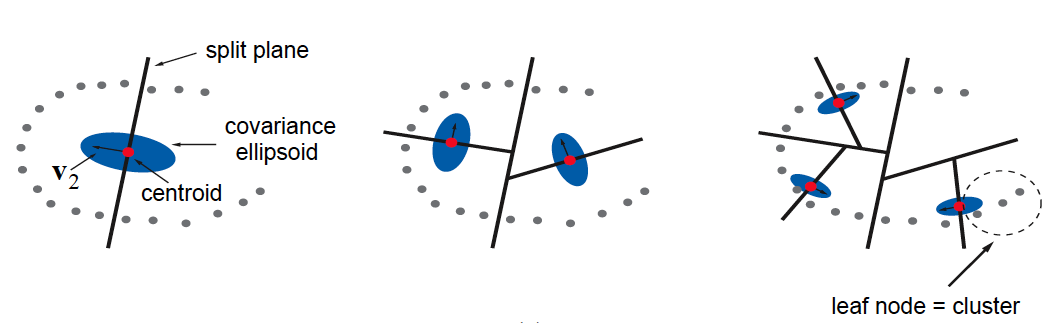
\includegraphics[width=\linewidth]{hierarchical_clustering}
  \caption{Classification hiérarchique~\cite{Pauly2002} \label{fig:sampling_hierarchical}}
\end{figure}

Afin de diviser l'espace, il est possible de faire appel à des structures de données tel que les \emph{Octrees} ou les \emph{Kd-Trees}, qui sont des cas particuliers de \emph{BSP}.

\subsection{Méthode iterative}
\begin{definition}[Sous-échantillonnage par simplification itérative]
  Méthode d'échantillonnage consistant à effectuer successivement l'une des étapes cités ci-dessous en fonction d'une mesure d'erreur quadratique:
  \begin{itemize}
    \item supprimer un point;
    \item fusionner une pair de points.
  \end{itemize}
\end{definition}

La première méthode génère une solution composé uniquement d'un sous-ensemble de points de $P$, autrement dit $P' \subseteq P$. Ceci peut engendré des effets indésirable sur la surface [FIXME: aliasing]. Pour palier à ce problème, il est préférable de fusionner des pairs de points.

\subsubsection{Méthode par suppression}
Une méthode présentée par \citeauthor{Alexa2001}~\cite{Alexa2001} consiste à évaluer la contribution d'un point $p_i$ à la surface $S$ issue du nuage de points $P$. Pour ce faire il faut comparer la surface $S$ et la surface $S'$ correspondant au nuage de points $P-\{p_i\}$. Une façon de procéder consisterait à calculer la distance de \emph{Hausdorff} [FIXME], mais pour des nuages contenant plusieurs millions de points, cela peut être trop coûteux en temps. Une approximation consiste à calculer la différence entre $p_i$ et sa projection sur $S'$ noté $p_i'$ [FIXME].\\

Une autre méthode proposé par \citeauthor{Linsen2001}~\cite{Linsen2001} est basé sur le même principe, mais détermine la contribution d'un point $p_i$ à l'aide d'une fonction pondérée $M(p_i)$ représentant la quantité d'information contenu par ce point.
$$M(p) := \alpha_d \cdot M_d(p)+\alpha_p \cdot M_p(p)+\alpha_c \cdot M_c(p)+\alpha_u \cdot M_u(p)+\alpha_{colour} \cdot M_{colour}(p)$$
où $M_d$ dépend de la distance de $p$ à ces voisins, $M_p$ de la non-planarité, $M_c$ de la variation des normales, $M_u$ de la variation non-uniforme de ces dernières, et $M_{colour}$ représente la variation de couleur entre $p$ et son voisinage.

\subsubsection{Méthode par fusion}
Cette méthode est une adaptation de celle présenté pour les maillages polygonaux~\cite{Hoppe1996}. Le principe consiste à placer les opérations de fusion dans une file de priorité suivant une mesure d'erreur. L'opération de fusion remplace deux point $p_1$ et $p_2$ par un nouveau point $\overline{p}$.

La mesure d'erreur présenté par \citeauthor{Pauly2002}~\cite{Pauly2002} est définie comme la somme des distances au carré entre le point $\overline{p}$ et l'ensemble des plans engendrés par $p_1$, $p_2$ et leurs voisins [FIXME:illustration].

\subsection{Methode par simulation}
\begin{definition}[Sous-échantillonnage par simulation de particule]
  Méthode d'échantillonnage consistant à calculer les nouvelles positions des points de l'ensemble $P'$ sur la surface $S$ en respectant des forces inter-particules.
\end{definition}

Cette technique fût initialement introduite par \citeauthor{Turk1992}~\cite{Turk1992} dans le domaine de la réduction de maillages polygonaux.

La première étape consiste à répandre aléatoirement de façon uniforme des points sur la surface. Afin de respecter la condition d'uniformité, il sera nécessaire déterminer la densité $\rho$. De cette façon, moins de points sont placé dans les zones à faible densité, et d'avantage dans le cas opposé [FIXME: calcul de $\rho$].

Dans un deuxième temps, la position de ces points est adapté à l'aide d'un algorithme de répulsion. Pour des raisons de rapidité, la force de rappel d'un point décroît linéairement en fonction de la distance. On parlera de \emph{rayon d'influence} fini. Le vecteur force est donc:
$$F_i(p)=k\cdot(r-\|p-p_i\|)\cdot(p-p_i)$$
où $F_i(p)$ est la force exercée par la particule $p$ sur la particule $p_i$, et $r$ est le \emph{rayon d'influence}.
La force totale exercée sur un point $p$ est donc définie par:
$$F(p)=\sum\limits_{i\in N_P}F_i(p)$$

Il est possible d'adapter la force de rappel en fonction d'autres paramètres, tel que la courbure. Pour ce faire, il faut remplacer le rayon d'influence $r$ par $\frac{r}{\sigma_n}$ ainsi que l'estimation de la densité $\rho$ par $\rho\cdot\sigma_n$ où $\sigma_n$ représente la variation de surface calculé à l'aide d'un voisinage de taille $n$.

Une fois la force $F(p)$ déterminée, il est nécessaire de déplacer le point $p$ tout en restant sur la surface $S$ décrite par le nuage de point $P$. Une solution tel qu'une projection \emph{MLS} est trop coûteuse en temps [FIXME].